\section{Специальный раздел}
\label{sec:special}

\subsection{Требования к разрабатываемой системе}

Требования к разрабатываемой системе представляют собой совокупность параметров и характеристик, которыми должно обладать разрабатываемое приложение для достижения поставленных целей и решения задач. Они определяют функциональность системы, ее поведение, а также условия, необходимые для ее корректной работы. Требования подразделяются на функциональные и нефункциональные.

Функциональные требования описывают специфические функции или действия, которые должна выполнять система. В контексте разрабатываемого приложения для поиска и возврата уянных вещей, это могут быть функции регистрации и авторизации пользователей, поиска утерянных вещей, добавления информации о утерянных вещах, связи между пользователями и системы уведомлений.

Нефункциональные требования определяют качественные характеристики системы, такие как производительность, безопасность, доступность, удобство использования, совместимость, масштабируемость, тестирование и документация.

Требования к разрабатываемой системе играют ключевую роль в процессе разработки приложения. Они служат основой для проектирования, реализации и тестирования системы. Без четко определенных требований невозможно разработать эффективное и надежное приложение, которое будет отвечать потребностям пользователей и бизнес-задачам.

В контексте курсовой работы на тему “Разработка приложения для поиска и возврата утерянных вещей”, требования к разрабатываемой системе позволяют сформулировать и структурировать задачи, которые должно решать приложение, а также определить параметры, необходимые для его успешной работы. Они служат основой для дальнейшего проектирования и разработки приложения, а также для оценки его эффективности и качества после внедрения.

\subsubsection{Функциональные требования}

\begin{itemize}
	\item Приложение должно предоставлять возможность регистрации и авторизации пользователей.
	\item Приложение должно предоставлять возможность поиска утерянных вещей по различным критериям (например, по типу вещи, по месту утери и т.д.).
	\item Пользователи должны иметь возможность добавлять информацию о утерянных вещах, включая описание, фотографии и место утери.
	\item Приложение должно предоставлять функционал для связи между пользователем, который нашел вещь, и пользователем, который ее потерял.
	\item Приложение должно иметь систему уведомлений, которая будет информировать пользователей о новых найденных вещах, соответствующих их критериям поиска.
\end{itemize}

ER-диаграмма представлена на рис.~\ref{fig:erd}.

\begin{figure}[htb]
	\centering
	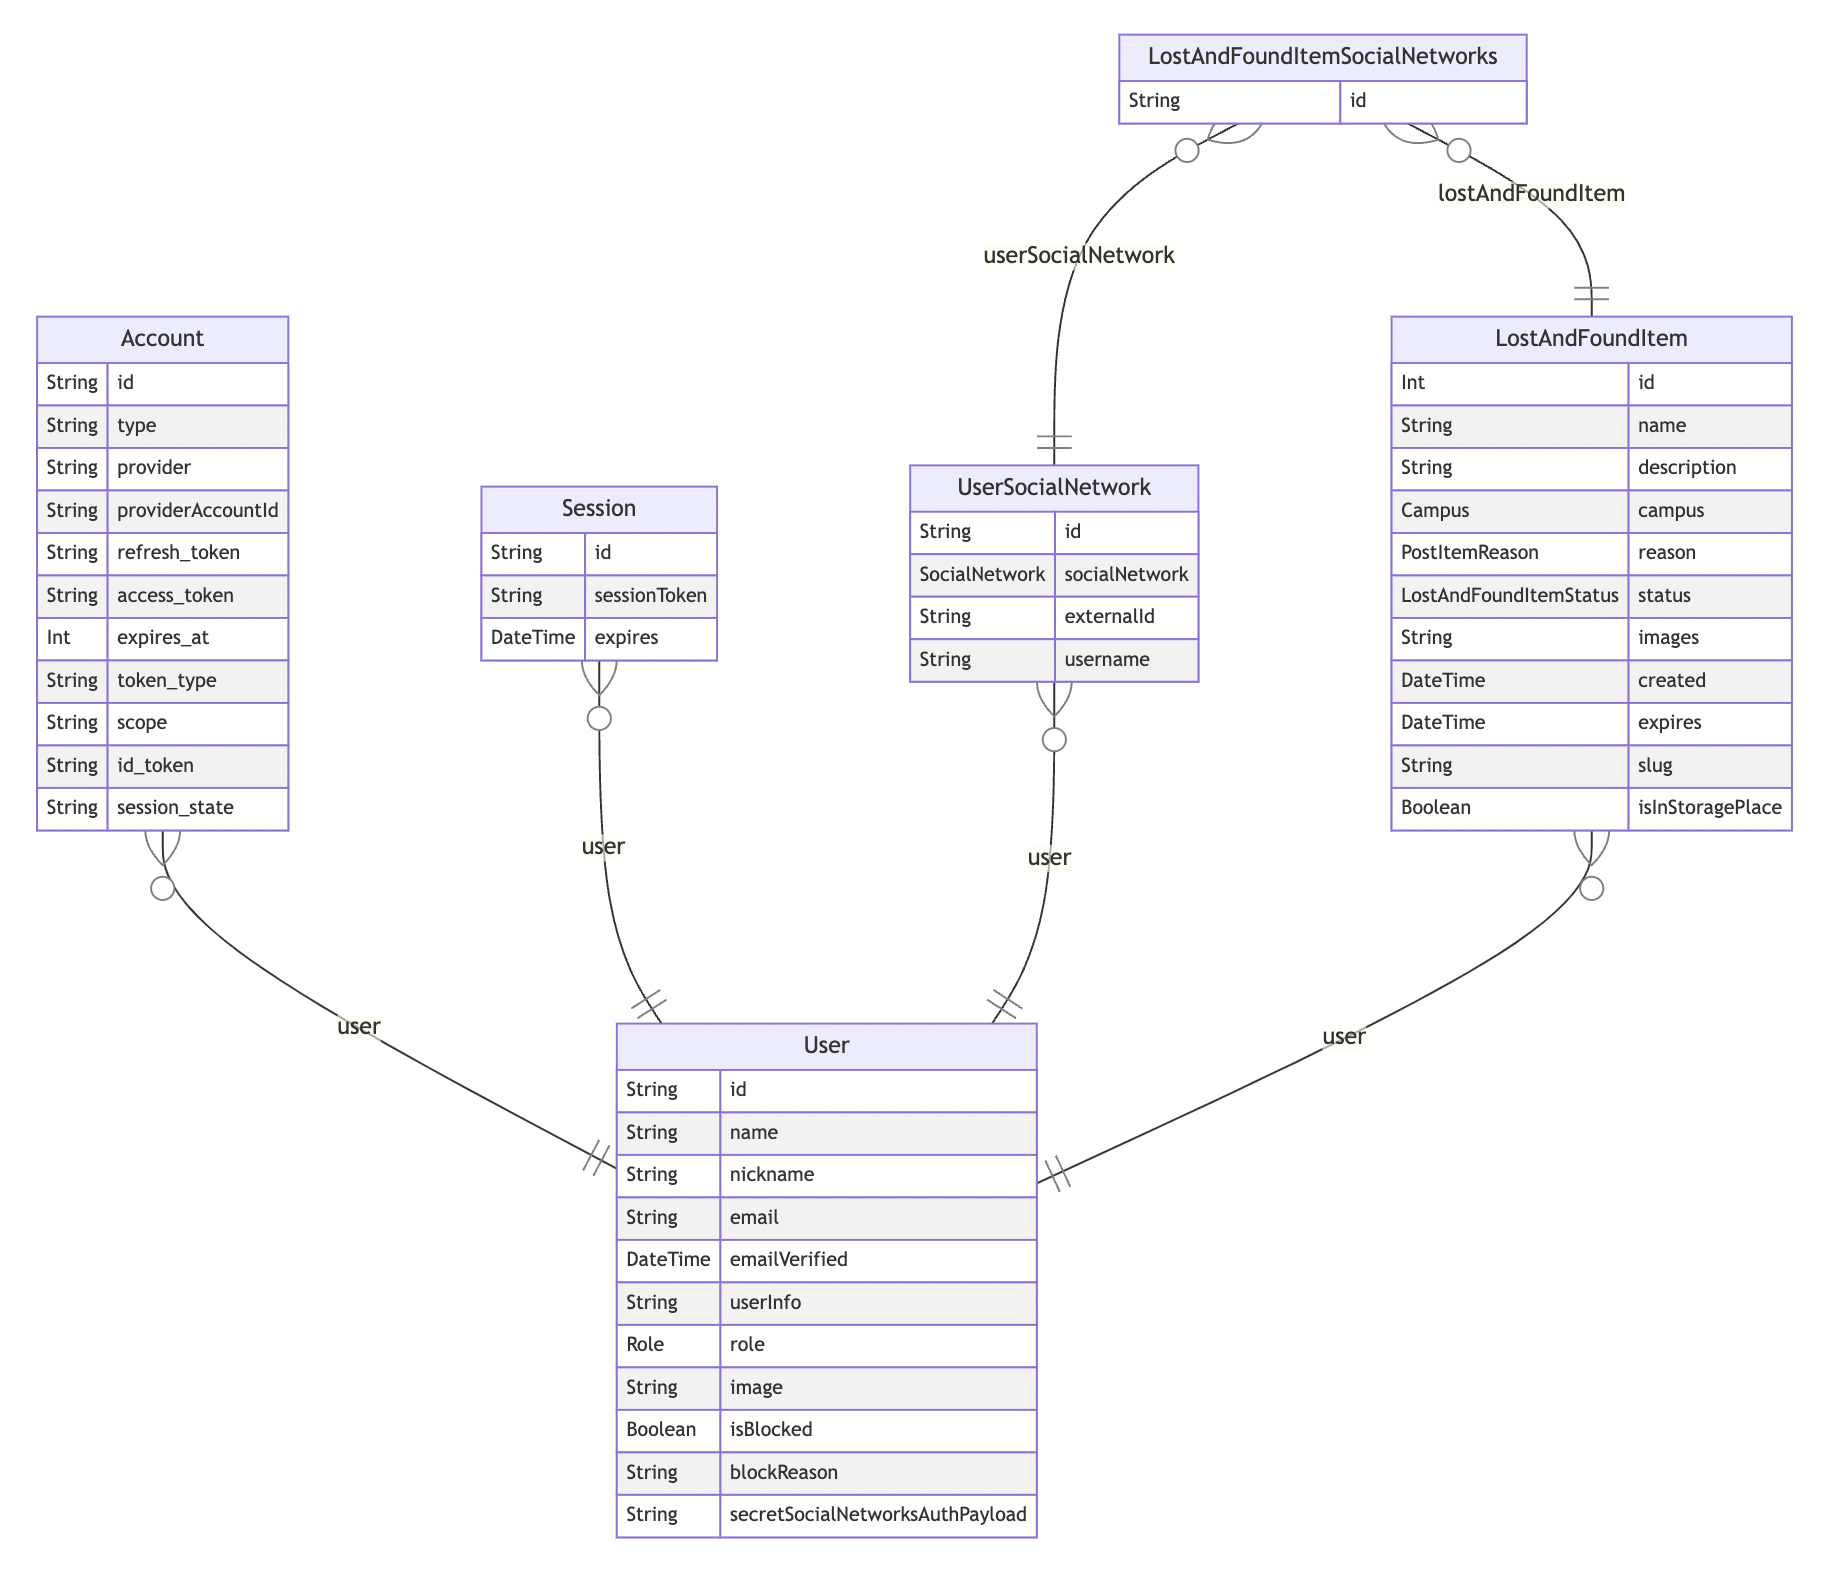
\includegraphics[width=.95\textwidth]{images/erd}
	\parskip=6pt
	\caption{ER-диаграмма системы}
	\label{fig:erd}
\end{figure}

\subsubsection{Нефункциональные требования}

\begin{itemize}
	\item Приложение должно обеспечивать быстрый поиск и отображение результатов, а также быстрое добавление информации о утерянных вещах.
	\item Все данные пользователей должны быть защищены. Пароли должны храниться в зашифрованном виде.
	\item Приложение должно быть доступно для использования 24/7.
	\item Интерфейс приложения должен быть интуитивно понятным и удобным для пользователей разного уровня компьютерной грамотности.
	\item Приложение должно быть совместимо с основными операционными системами (iOS, Android) и браузерами (Chrome, Firefox, Safari, Edge).
	\item Приложение должно быть способно обслуживать большое количество пользователей одновременно без снижения производительности.
	\item Приложение должно быть тщательно протестировано на наличие ошибок и уязвимостей перед запуском.
\end{itemize}

\subsection{Проектирование модулей автоматизации процессов}

Проектирование модулей автоматизации процессов включает в себя разработку структуры и функционала модулей, которые будут автоматизировать ключевые процессы приложения для поиска и возврата утерянных вещей. В данном случае, ключевыми процессами являются: регистрация и авторизация пользователей, добавление и поиск утерянных вещей, связь между пользователями и система уведомлений.

\subsubsection{Модуль регистрации и авторизации пользователей}

Этот модуль предназначен для создания и поддержки учетных записей пользователей. Он должен включать функции регистрации, авторизации и восстановления пароля. Для обеспечения безопасности, пароли должны храниться в зашифрованном виде.

\subsubsection{Модуль бесконечных лент объявлений потерянных, найденных вещей}

Модуль бесконечных лент объявлений представляет собой ключевой элемент приложения для поиска и возврата утерянных вещей. Он предназначен для отображения объявлений о потерянных и найденных вещах в формате бесконечной ленты, обеспечивая пользователю удобный и непрерывный доступ к информации.

\subsubsection{Модуль добавления и поиска утерянных вещей}

Этот модуль отвечает за добавление информации о утерянных вещах в базу данных и поиск по этой базе. Он должен предоставлять пользователю возможность добавлять описание, фотографии и место утери вещи, а также осуществлять поиск по различным критериям.

\subsubsection{Модуль генерации описания объявлений}

Модуль генерации описания объявлений является важным компонентом приложения для поиска и возврата утерянных вещей. Он предназначен для автоматического создания описаний объявлений на основе введенных пользователем данных, что облегчает процесс создания объявлений и повышает их качество.

\subsection*{Вывод по разделу}

Проектирование модулей автоматизации процессов является важным этапом в разработке приложения для поиска и возврата утерянных вещей. Каждый из модулей, включая модуль регистрации и авторизации пользователей, модуль бесконечных лент объявлений, модуль добавления и поиска утерянных вещей и модуль генерации описания объявлений, играет свою уникальную роль в обеспечении функциональности и эффективности приложения.

Каждый из этих модулей важен для обеспечения эффективности и удобства использования приложения, и их совместная работа позволяет создать надежное и функциональное приложение для поиска и возврата утерянных вещей.